\chapter{Risk, Reward and Arbitrage}


\section{Capital Asset Pricing Model (CAPM)}

\subsection{Valuation}

\begin{definition}
    Valuation is the analytical process of determining the current (or projected) worth of an asset or a company. \\
    \textbf{Components of a valuation:}
    \begin{itemize}
        \item \textbf{Projected cash flows:} The expected future cash flows of the asset or company.
        \item \textbf{Interest/hurdle rate:} The rate of return required by the investor to invest in the asset or company.
    \end{itemize}
\end{definition}

\begin{definition}
    [Pricing Risk]
    Pricing risk is the process of determining the appropriate interest rate (rate of return) for an asset or company based on the risk associated with the asset or company.
\end{definition}

\begin{theorem}
    [Project/Company Returns]
    Say you have a portfolio of $n$ stocks, and the price of the $i^{th}$ stock is given in table \ref{tab:time_period_price}. The returns of a project/company (stock) at time $t_j$ is given by:
    \begin{equation}
        P_{t_j} = P_{t_{j-1}} e^{r_{t_{j}}\Delta t}
    \end{equation}
    Because we are dealing with continuous compounding.\\
    We can find the rate of return $r_{t_{j}}$ by:
    \begin{equation}
        r_{t_{j}} = \frac{1}{\Delta t} \ln\left(\frac{P_{t_j}}{P_{t_{j-1}}}\right)
    \end{equation}
    The return vector for the $i^{th}$ stock is given by:
    \begin{equation}
        \overrightarrow{R_i} =  \begin{bmatrix}
            r_{t_1} \\
            r_{t_2} \\
            \vdots  \\
            r_{t_n}
        \end{bmatrix}
    \end{equation}
\end{theorem}

\begin{table}[h!]
    \centering
    \begin{tabular}{|c|c|}
        \hline
        \textbf{Time Period (t)} & \textbf{Price (P)} \\ \hline
        0                        & 20                 \\ \hline
        1                        & 21                 \\ \hline
        2                        & 22                 \\ \hline
        3                        & 20                 \\ \hline
        4                        & 21                 \\ \hline
    \end{tabular}
    \caption{Time Period vs. Price}
    \label{tab:time_period_price}
\end{table}

\begin{definition}
    [Volatility]
    Volatility is a statistical measure of the dispersion of returns for a given security or market index.
    Volatility is the standard deviation of the returns.
    \begin{equation}
        \sigma = \sqrt{Var(\overrightarrow{R_i})} = \sqrt{\frac{1}{n-1} \sum_{i=1}^{n} (r_i - \bar{r})^2}
    \end{equation}
    where:
    \begin{itemize}
        \item $r_i$ is the return at time $i$.
        \item $\bar{r}$ is the average return.
        \item $n$ is the number of returns.
    \end{itemize}
\end{definition}

\begin{proposition}
    [Modern Portfolio Theory]
    \textbf{Objective:} To maximize the expected return, while minimizing volatility/risk ($\sigma$).\\
\end{proposition}
\begin{definition}
    [Covariance]
    The covariance between two assets is a measure of how the two assets move together. If the covariance is positive, the assets move together, i.e. when one asset increases, the other asset also increases.
    \begin{equation}
        Cov(\overrightarrow{R_i},\overrightarrow{R_j}) = \frac{1}{n-1} \sum_{i=1}^{n} (r_{i} - \bar{r_i})(r_{j} - \bar{r_j})
    \end{equation}
\end{definition}

\begin{lemma}
    [Purpose of Covariance]
    Having positive covariances across your assets should increase your volatility, because if one crashes, the others are likely to crash as well. So in general, we want negative, or at least low, covariances.\\
\end{lemma}

\begin{definition}
    Assume we can proportionally invest in $x_i$ amount in the $i^{th}$ asset. We define:
    \begin{equation}
        \overrightarrow{X} = \begin{bmatrix}
            x_1    \\
            x_2    \\
            \vdots \\
            x_n
        \end{bmatrix}
    \end{equation}
    And the covariance matrix of the returns of the $n$ assets is given by:
    \begin{equation}
        \Sigma = \begin{bmatrix}
            \sigma_{11} & \sigma_{12} & \cdots & \sigma_{1n} \\
            \sigma_{21} & \sigma_{22} & \cdots & \sigma_{2n} \\
            \vdots      & \vdots      & \ddots & \vdots      \\
            \sigma_{n1} & \sigma_{n2} & \cdots & \sigma_{nn}
        \end{bmatrix}
    \end{equation}
    Where:
    \begin{itemize}
        \item $\sigma_{ij} = \sigma_{ji} = Cov(\overrightarrow{R_i},\overrightarrow{R_j})  $ is the covariance between the $i^{th}$ and $j^{th}$ asset.
        \item $\sigma_{ii} = Var(\overrightarrow{R_i})$ is the variance of the $i^{th}$ asset.
    \end{itemize}
\end{definition}


\begin{definition}
    [Portfolio Expected Return]
    The expected return of a portfolio is given by:
    \begin{equation}
        \mathbb{E}[\overrightarrow{R_p}] = x_1 \mathbb{E}[\overrightarrow{R_1}] + x_2 \mathbb{E}[\overrightarrow{R_2}] + \cdots + x_n \mathbb{E}[\overrightarrow{R_n}] = \sum_{i=1}^{n} x_i \mathbb{E}[\overrightarrow{R_i}]
    \end{equation}
    Where:
    \begin{itemize}
        \item $\mathbb{E}[\overrightarrow{R_i}]$ is the expected return of the $i^{th}$ asset.
        \item $\mathbb{E}[\overrightarrow{R_p}]$ is the expected return of the portfolio.
        \item $\overrightarrow{R_i}$ is the historical return of the $i^{th}$ asset.
        \item $x_i$ is the proportion of the $i^{th}$ asset in the portfolio.
    \end{itemize}
    Intuitively, the expected return of each asset is multiplied by how much of the asset is in the portfolio.
\end{definition}

\begin{definition}
    [Portfolio Volatility]
    The volatility of a portfolio is given by:
    \begin{equation}
        \sigma_p = \sqrt{\overrightarrow{X}^T \times \Sigma \times \overrightarrow{X}}
    \end{equation}
\end{definition}

\begin{corollary}
    [Maximization]
    We want to maximize the expected return of the portfolio ($\mathbb{E}[\overrightarrow{R_p}]$) while minimizing the volatility of the portfolio ($\sigma_p$).\\
\end{corollary}

\begin{theorem}
    [CAPM Assumption]
    The Capital Asset Pricing Model (CAPM) assumes that investors are rational and risk-averse, in addition, it is just a model with numerous assumptions.\\
    \textbf{Assumptions:}
    \begin{itemize}
        \item Correlation and volatility of and between assets are fixed and constant forever
        \item All investors aim to maximize economic utility (i.e. make as much money as possible, regardless of any other considerations)
        \item[] \begin{itemize}
                  \item Although usually true, we see irrational behavior in the market (e.g. driven by fear)
              \end{itemize}
        \item All investors are rational and risk-averse
        \item All investors have access to the same information at the same time
        \item Investors have accurate conception of possible returns, i.e. the probability beliefs of investors match the true distribution of returns.
        \item There are no taxes or transaction costs
        \item[] \begin{itemize}
                  \item Often they are negligible, so they are ignored
              \end{itemize}
        \item All investors are price takers, i.e. their actions do not influence prices
        \item Any investor can lend and borrow an unlimited amount at the risk free rate of interest
        \item All securities can be divided into parcel of any size
    \end{itemize}
\end{theorem}

\begin{definition}
    [Efficiency Frontier]
    The efficiency frontier is the set of portfolios (expected returns and their respective volatilities, $\{(\mathbb{E}[R_p], \sigma_p)\}$) that satisfy the following conditions:
    \begin{align*}
        \text{Minimize:}   & \quad \sigma_p^2 = \overrightarrow{X}^T \Sigma \overrightarrow{X} \\
        \text{Subject to:} & \quad \sum_{i=1}^{n} x_i = 1                                      \\
                           & \quad \sum_{i=1}^{n} x_i \mathbb{E}[R_i] = \mathbb{E}[R_p]        \\
                           & \quad \sum_{i=1}^{n} x_i \sigma_i = \sigma_p
    \end{align*}
    Because $\sigma_p$ is squared, we can expect a parabolic shape for the curve. But the efficiency frontier is always the top half of the parabola, because we prefer a portfolio with a higher return for the same volatility.
\end{definition}
\begin{figure}[h!]
    \centering
    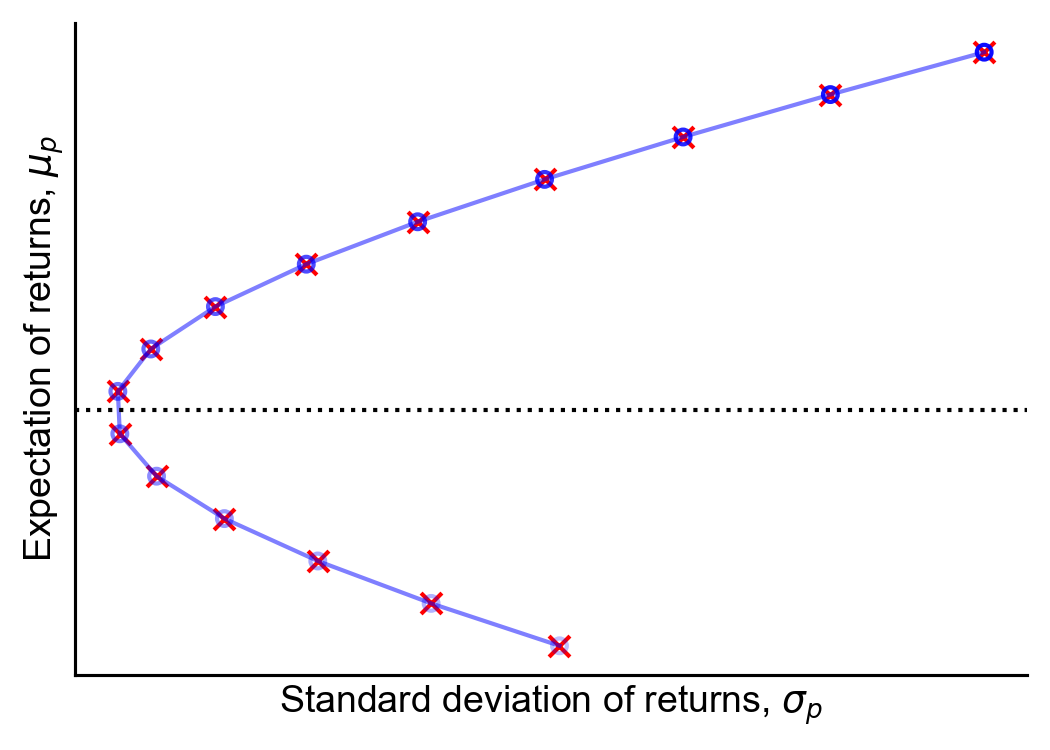
\includegraphics[width=0.6\textwidth]{LECTURE_4/efficient_frontier.png}
    \caption{Efficient Frontier}
    \label{fig:efficient_frontier}
\end{figure}

\begin{definition}
    [Tangency/Market Portfolio and Capital Market Line]
    Now we want to find the largest ratio of \textbf{excess} return to risk ($\frac{\mathbb{E}[R_p]}{\sigma_p}$).
    So we draw a tangent line that also intersects at the risk-free rate, $r_f$, this line is called the Capital Market Line (CML). The point where the tangent line intersects the efficient frontier is called the Tangency/Market Portfolio.\\
\end{definition}

\begin{definition}
    [Sharpe Ratio]
    To prove that this provides the largest ratio of excess return to risk, we realize that the slope of the tangent line is given by:
    \begin{align*}
        m & = \frac{y_2 - y_1}{x_2 - x_1}                \\
        m & = \frac{\mathbb{E}[R_p] - r_f}{\sigma_p - 0}
    \end{align*}
    This is the Sharpe Ratio, we want to maximize it, and it is the slope of the tangent line.\\
    Higher the slope, higher the sharpe ratio, higher the excess return for the same risk.
\end{definition}

\begin{figure}[h!]
    \centering
    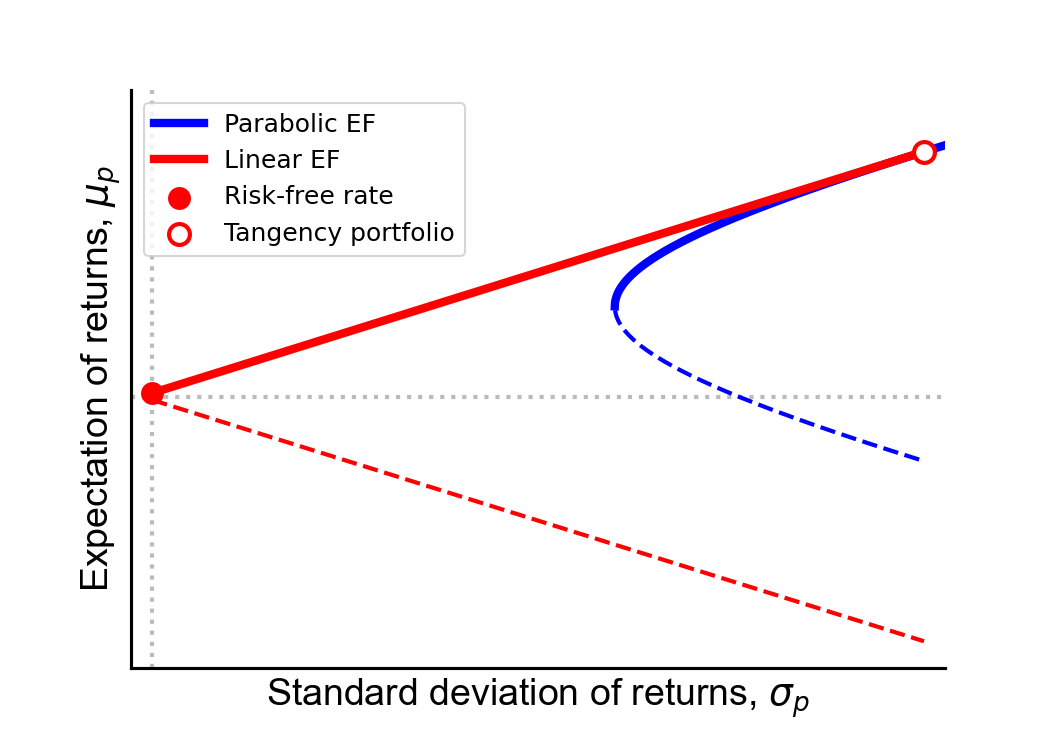
\includegraphics[width=0.6\textwidth]{LECTURE_4/CML.png}
    \caption{Capital Market Line}
    \label{fig:capital_market_line}

\end{figure}

\begin{proposition}
    [Leveraging Down/ Deleveraging]
    If we invest $50\%$ in the risk-free asset and $50\%$ in the market portfolio, we expect a return that is the average of the two returns, and a volatility that is the average of the two volatilities.\\
    \begin{equation}
        \mathbb{E}[R_{p}] = w\cdot \mathbb{E}[R_{m}] + (1-w)\cdot r_f
    \end{equation}

    \begin{equation}
        \sigma_{p} = \sqrt{w^2 \sigma_{m}^2 + (1-w)^2 \cdot \sigma_{f}}, \quad \sigma_{f} = 0
    \end{equation}
    Where $w$ is the weight of the market portfolio.\\
    This is called leveraging down, because we are investing in a less risky portfolio than the market portfolio.\\
\end{proposition}

\begin{lemma}
    Note that this can be done with any two points on the CML, not just the risk-free rate and the market portfolio.
\end{lemma}

\begin{proposition}
    [Leveraging Up]
    If we invest $150\%$ in the market portfolio and $-50\%$ (borrowing) in the risk-free asset, we expect a return that is $50\%$ higher than the market portfolio, and a volatility that is $50\%$ higher than the market portfolio.\\
    This is called leveraging up, because we are investing in a more risky portfolio than the market portfolio.\\
\end{proposition}


\begin{remark}
    It may seem weird at first that investing higher than the market portfolio suggests that we borrowed money at the risk-free rate. But this is just how the CAPM models riskier investments. This is because, in theory, no one would invest higher than the market portfolio, so the only way to achieve a higher return is to borrow money at the risk-free rate and invest more in the market portfolio.\\
\end{remark}

\begin{definition}
    [Stock Index]
    A stock index is a measure of the value of a section of the stock market. When the CAPM is applied to the stock market, the market portfolio is the stock index.\\
\end{definition}

\begin{definition}
    [Systematic Risk]
    Systematic risk is the risk that is inherent to the entire market or market segment. It is also known as undiversifiable risk or market risk $\beta$.\\
    E.g. If the economy is in a recession, all stocks will likely decrease in value.\\
\end{definition}

\begin{definition}
    [Idiosyncratic Risk]
    Idiosyncratic risk is the risk that is specific to a particular company or industry. It can be mitigated through diversification.\\
    E.g. If a company's CEO is caught embezzling money, the company's stock will likely decrease in value.\\
\end{definition}

\begin{proposition}
    You can 'portfolio' away idiosyncratic risk by diversifying your portfolio, but not systematic risk.\\
    \textbf{In the CAPM model, we assume everyone is logical and diversifies away idiosyncratic risk. So we only care about systematic risk.}
\end{proposition}

\begin{theorem}
    [Expected Return of an asset]
    The expected return of an asset is given by:
    \begin{equation}
        \mathbb{E}[R_i] = r_f + \beta_i(\mathbb{E}[R_m] - r_f)
    \end{equation}
    Intuitively, it says that the expected return of an asset is the risk-free rate plus the amount that an increase in the market portfolio would increase the return of the asset.\\
    The systematic risk of the asset is defined as:
    \begin{equation}
        \beta_i = \frac{Cov(R_i,R_m)}{Var(R_m)} = \frac{\sigma_{i,m}}{\sigma_{m}^2} = \frac{\rho_{i,m} \sigma_i}{\sigma_{m}}
    \end{equation}
    Plotting $\mathbb{E}[R_i]$ vs. $\beta_i$ gives the Security Market Line (SML).\\
\end{theorem}

\begin{figure}[h!]
    \centering
    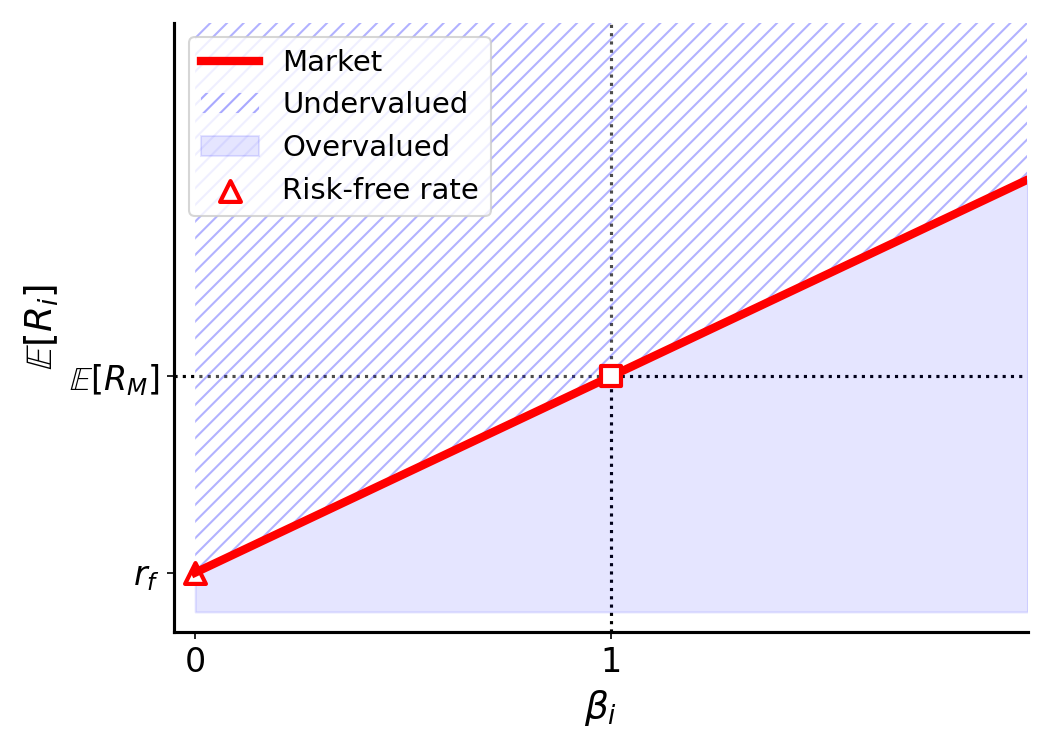
\includegraphics[width=0.6\textwidth]{LECTURE_4/SML.png}
    \caption{Security Market Line}
    \label{fig:security_market_line}
\end{figure}

\begin{example}
    Given the following market and company X data, estimate the expected stock return for company X:
    \begin{itemize}
        \item Market data
              \begin{itemize}
                  \item Risk-free rate: $2\%$
                  \item Expected market return: $8\%$
                  \item Market volatility: $10\%$
              \end{itemize}
        \item Company X data
              \begin{itemize}
                  \item Historical stock price return correlation to the market: $0.6$
                  \item Historical stock price volatility: $0.15$
              \end{itemize}
    \end{itemize}
    \textbf{Solution:}

    We can find the expected return of company X by:
    \begin{align*}
        \beta_i         & = \frac{\rho_{i,m} \sigma_i}{\sigma_{m}} = \frac{0.6 \cdot 0.15}{0.1} = 0.9 \\
        \mathbb{E}[R_i] & = r_f + \beta_i(\mathbb{E}[R_m] - r_f) = 0.02 + 0.9(0.08 - 0.02) = 0.074
    \end{align*}
\end{example}

\begin{definition}
    A company with a beta of 0.9 has a stock price that is currently trading at \$170 dollars a share. The current risk-free rate is 2\%, and the market rate is 7\%. What is the expected price of a share 5 years from now, if the company pays no dividends?\\

    \textbf{Solution:}

    We can find the expected return of the stock by:
    \begin{align*}
        \mathbb{E}[R_i] & = r_f + \beta_i(\mathbb{E}[R_m] - r_f) = 0.02 + 0.9(0.07 - 0.02) = 0.065        \\
        P_{t_0}         & = 170                                                                           \\
        P_{t_5}         & = P_{t_0} e^{r_{t_5} \cdot 5} = 170 e^{0.065 \cdot 5} = 170 e^{0.325} = \$235.3
    \end{align*}
\end{definition}


\begin{example}
    Consier a stock that has a current share price of \$10 and pays quarterly dividends of \$0.10 per share. Determine the expected stock price 3 years from now given the following:
    \begin{itemize}
        \item Expected market return: $10\%$
        \item Risk-free rate: $3\%$
        \item Company beta: $1.2$
    \end{itemize}

    \textbf{Solution:}

    We can find the expected return of the stock by:
    \begin{align*}
        \mathbb{E}[R_i] & = r_f + \beta_i(\mathbb{E}[R_m] - r_f) = 0.03 + 1.2(0.1 - 0.03) = 0.114
    \end{align*}
    We know that this gives us yearly effective compounding rate. We also want the quarterly compounding rate, per quarter:
    \begin{align*}
        (1 + 0.114)^{\frac{1}{4}} & = (1 + 0.114) \\
        r_{t_1}                   & = 0.02736
    \end{align*}
    Next we draw the cash-flow diagram for the stock:
    \begin{figure}[h!]
        \centering
        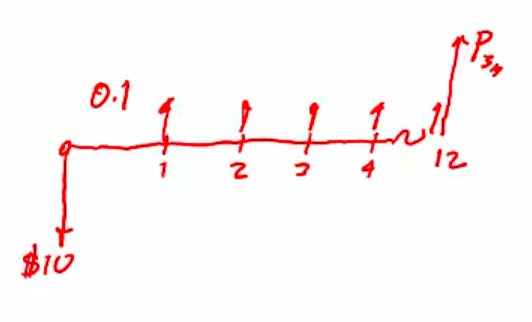
\includegraphics[width=0.6\textwidth]{LECTURE_4/cash-flow.png}
        \caption{Cash Flow Diagram}
        \label{fig:cash_flow_diagram}
    \end{figure}
    So we can model the diagram as:
    \begin{align*}
        P_0   & = \$0.1(P/A, 0.02736, 12) + P_3(P/F, 0.02736, 12) \\
        P_{3} & = \$ 12.43
    \end{align*}
\end{example}

\section{Arbitrage and Replicating Portfolio Diagrams}

\begin{definition}
    [Arbitrage]
    Arbitrage is the simultaneous purchase and sale of an asset to profit from a difference in the price. It is a trade that profits by exploiting the price differences of identical or similar financial instruments on different markets or in different forms.\\

    It occurs when there is an opportunity to achieve a risk-free gain at a rate of return that is higher than the risk-free rate.\\
\end{definition}

\begin{definition}
    [No Arbitrage Assumption (No Free Lunch)]
    The no-arbitrage assumption states that there are no risk-free profit opportunities in a perfect market.\\
\end{definition}


\begin{definition}
    [Forward/Futures Contract]
    A forward contract is a contract between two parties to buy or sell an asset at a specified future date at a price agreed upon today.\\

    A futures contract is the same, except it is traded on an exchange (thus, often less customized to any particular party).\\
\end{definition}

\begin{example}
    Say you could buy a bushel of corn for \$10 today and enter into a forward contract to deliver the corn for a pre-settled price of \$12 per bushel one year from now- assume it costs you nothing to store the corn. Say you could also borrow at 10\%.\\
    Is this an arbitrage opportunity?\\
    And what is the no-arbitrage price of corn (assuming the future price of corn is still \$12)?\\

    \textbf{Solution:}

    First we draw the cash-flow diagram for the situation:
    \begin{figure}[h!]
        \centering
        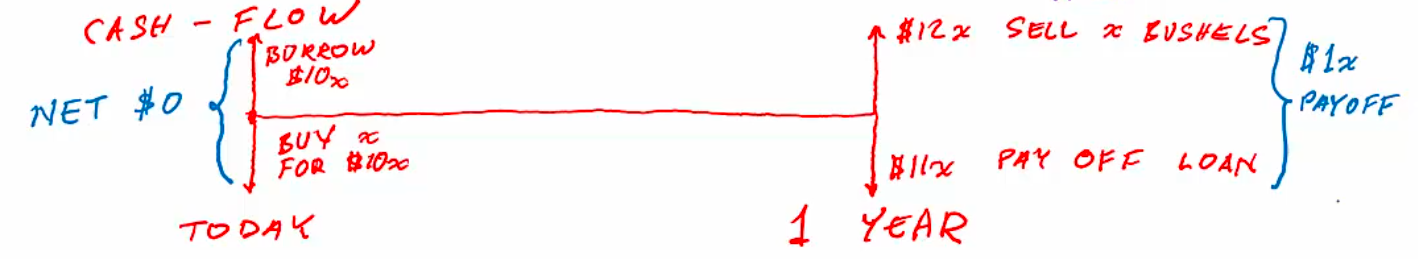
\includegraphics[width=0.6\textwidth]{LECTURE_4/cash-flow-2.png}
        \caption{Cash Flow Diagram}
        \label{fig:cash_flow_diagram_2}
    \end{figure}

    \begin{align*}
        F = +12 - 10(1+0.1) = 1
    \end{align*}
    So this is an arbitrage opportunity, because you can make a risk-free profit of \$1. In theory we should invest as much as possible in this opportunity, but in reality, laws of supply and demand will prevent this from happening.\\
    The no-arbitrage price of the forward contract can be found by:
    \begin{align*}
        P = \frac{12}{1+0.1} = \$10.91
    \end{align*}
    At this point there is no profit to be made.
\end{example}

\begin{example}
    Given an interest rate yield curve, determine the appropriate forward rate, $r_{t_1}$, that one could lock into today for specified interest rate from time $t_1$ to time $t_2$.\\
    \begin{figure}[h!]
        \centering
        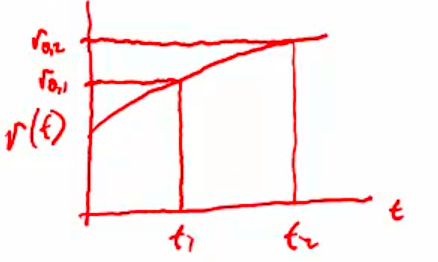
\includegraphics[width=0.6\textwidth]{LECTURE_4/interest-rate-curve.png}
        \caption{Interest Rate Curve}
        \label{fig:interest_rate_curve}
    \end{figure}

    \textbf{Solution:}

    We can use the \textbf{no-arbitrage assumption} to find two ways to get from $t_1$ to $t_2$ and equate them:
    \begin{align*}
        t = t_1 : \quad & F_1 = P_0e^{r_{0,1}t_1}                 \\
        t = t_2 : \quad & F_2 = F_1e^{r_{t_1,t_2}(t_2-t_1)}       \\
                        & F_2^{\prime} = F_1 e^{r_{1,2}(t_2-t_1)}
    \end{align*}
    The no-arbitrage assumption states that $F_2 = F_2^{\prime}$, so we can equate the two equations to find the forward rate:
    \begin{align*}
        F_2                                       & = F_2^{\prime}                          \\
        P_0e^{r_{0,1}t_1}e^{r_{t_1,t_2}(t_2-t_1)} & = P_0e^{r_{0,1}t_1}e^{r_{1,2}(t_2-t_1)} \\
        r_{1,2} = \frac{r_{0,1}t_1 + r_{t_1}}{t_2 - t_1}
    \end{align*}
\end{example}

\begin{example}
    [Using Replication to Price an Asset]
    \label{ex:replication}
    What is a fair price for a project whose payoff is \$140 if the market goes up and \$30 if the market goes down?\\
    \begin{itemize}
        \item The risk-free rate is 5\% for this period
        \item The current market portfolio is priced at \$100
        \item If the market goes up, it will be worth \$120
        \item If the market goes down, it will be worth \$95
    \end{itemize}
    If the probability of the market going up is 60\%, what is the expected return on the market portfolio? What is the expected return of the project?\\
    What if the expected payoff of the project was \$140, regardless of what the market did?\\

    \textbf{Solution:}

    The project can be modeled by the following diagram:


    \begin{figure}[h!]
        \centering
        \begin{subfigure}[b]{0.4\textwidth}
            \centering
            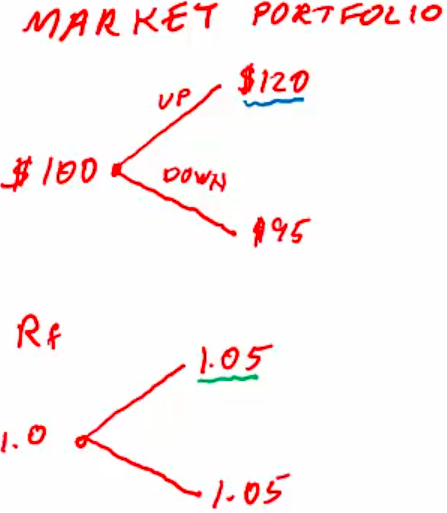
\includegraphics[width=\textwidth]{LECTURE_4/rep1.png}
            \caption{Market Portfolio Diagram}
            \label{fig:market_portfolio_diagram}
        \end{subfigure}
        \hfill
        \begin{subfigure}[b]{0.4\textwidth}
            \centering
            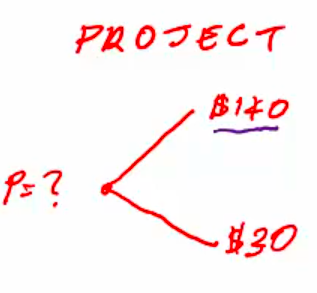
\includegraphics[width=\textwidth]{LECTURE_4/rep2.png}
            \caption{Project Diagram}
            \label{fig:project_diagram}
        \end{subfigure}

    \end{figure}
    We can solve for the for the factor $a, b$ that would make the project equivalent to the market portfolio:
    \begin{align*}
        \text{Up: }   & 140 = a \cdot 120 + b \cdot 1.05 \\
        \text{Down: } & 30 = a \cdot 95 + b \cdot 1.05
    \end{align*}
    Solving for $a, b$ gives us:
    \begin{align*}
        a & = 4.4    \\
        b & = -369.5
    \end{align*}
    So we can use this factors to find the present value of the project:
    \begin{align*}
        P_0 & = 4.4 \cdot 100 - 369.5 \cdot 1.00 = \$ 70.48
    \end{align*}
    Note: the probabilty of the market going up was not considered in this calculation.\\

\end{example}

\begin{definition}
    [Expected Value]
    The expected value of a project is the weighted average of the possible outcomes of the project, where the weights are the probabilities of the outcomes.\\
    \begin{equation}
        \mathbb{E}[P] = \sum_{i=1}^{n} P_i \cdot p_i
    \end{equation}
    Where:
    \begin{itemize}
        \item $P_i$ is the possible outcome of the project.
        \item $p_i$ is the probability of the outcome.
    \end{itemize}
\end{definition}

\begin{definition}
    [Expected Future Payoff/Return]

    The expected future payoff of the project is given by the expected value of the project, over the present value of the project:

    \begin{equation}
        \mathbb{E}[R] = \frac{\mathbb{E}[P]}{P_0} -1 = \frac{\sum_{i=1}^{n} P_i \cdot p_i}{P_0} -1
    \end{equation}

\end{definition}

\begin{example}
    Using the data from example \ref{ex:replication}, given that the probability of the market going up is $60\%$, what is the expected return of the market portfolio? What is the expected return of the project? And what is the systematic risk of the project?\\

    \textbf{Solution:}

    We can find the expected return of the market portfolio by:

    \begin{align*}
        \mathbb{E}[R_m] & = \frac{120\cdot 0.6 + 95\cdot 0.4}{100} - 1 = 0.1 = 10\%
    \end{align*}

    We can find the expected return of the project by:

    \begin{align*}
        \mathbb{E}[R_p] & = \frac{140\cdot 0.6 + 30\cdot 0.4}{70.48} - 1 = 36.2\%
    \end{align*}

    We can find the systematic risk of the project by:

    \begin{align*}
        \mathbb{E}[R_p] & = r_f + \beta_i(\mathbb{E}[R_m] - r_f) \\
        0.362           & = 0.05 + \beta_i(0.1 - 0.05)           \\
        \beta_i         & = 6.4
    \end{align*}
\end{example}

\begin{example}
    Again using the data from example \ref{ex:replication}, what would the present price be, given the expected payoff of the project was \$140, regardless of what the market did? And what would the present value be, if the project payoff was independent of the market, such that there was a 50\% chance of \$150, and a 50\% chance of \$130?\\

    \textbf{Solution:}

    This would mean the project is risk-free, and assuming no-arbitrage, we would simply discount to the present value using the risk-free rate (also, the systematic risk would be zero). So the present value of the project would be:
    \begin{align}
        P_0 & = \frac{140}{1.05} = \$133.33
    \end{align}

    We know $\beta = 0$, because there's no relation with the market conditions. So:
    \begin{align}
        \mathbb{E}[P] & = 150\cdot 0.5 + 130\cdot 0.5 = \$140 \\
    \end{align}
    And the present value of the project would be:
    \begin{align}
        P_0 & = \frac{140}{1.05} = \$133.33
    \end{align}

\end{example}


\begin{example}
    [Pricing an Asset with both Systematic and Idiosyncratic Risk]

    A wealthy (risk-neutral) investor has an opportunity to invest in a product development project. The outcome of the technology is uncertain, there is a 60\% chance that the technology works very well and a 40\% chance it will not meet all expectations. If the market goes up:
    \begin{itemize}
        \item And the technology works very well (60\% probability) the payoff will be \$80k
        \item Otherwise the payoff will be \$50k (technology did meet all expectations)
    \end{itemize}
    If the market goes down:
    \begin{itemize}
        \item And the technology works very well (60\% probability) the payoff will be \$55k
        \item Otherwise the payoff will be \$20k (technology did meet all expectations)
    \end{itemize}
    Other details include:
    \begin{itemize}
        \item Current market portfolio is \$45
        \item If the market goes up, payoff of the market portfolio will be \$60
        \item If the market goes down, payoff of the market portfolio will be \$40
        \item Risk-free rate is 5\%
        \item An initial investment of \$20k is required for the project
    \end{itemize}
    How much should the investor pay for the project?\\

    \textbf{Solution:}
    We can model the project with the following diagrams:

    \begin{figure}[h!]
        \centering
        \begin{subfigure}[b]{0.4\textwidth}
            \centering
            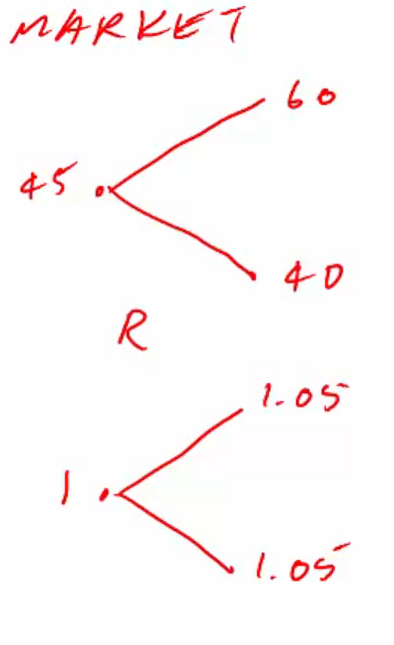
\includegraphics[width=\textwidth]{LECTURE_4/rep4.png}
            \caption{Market Portfolio Diagram}
            \label{fig:idiosyncratic_market_portfolio_diagram}
        \end{subfigure}
        \hfill
        \begin{subfigure}[b]{0.4\textwidth}
            \centering
            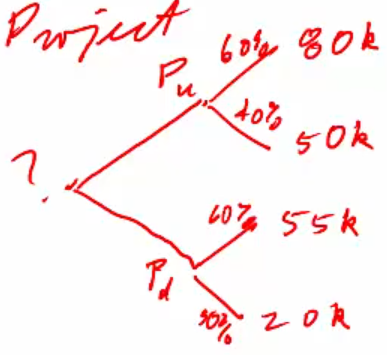
\includegraphics[width=\textwidth]{LECTURE_4/rep3.png}
            \caption{Project Diagram}
            \label{fig:idiosyncratic_project_diagram}
        \end{subfigure}

    \end{figure}

    We can first solve for the expected values of the project if the market goes up and down:
    \begin{align*}
        \mathbb{E}[P] & = \$80k \cdot 0.6 + \$50k \cdot 0.4 = \$68k \\
        \mathbb{E}[P] & = \$55k \cdot 0.6 + \$20k \cdot 0.4 = \$41k
    \end{align*}
    Now we can solve for $a, b$ that would make the project equivalent to the market portfolio:

    \begin{align*}
        \text{Up: }   & \$68k = a \cdot 60 + b \cdot 1.05 \\
        \text{Down: } & \$41k = a \cdot 40 + b \cdot 1.05
    \end{align*}

    Solving for $a, b$ gives us:
    \begin{align*}
        a & = 1.35k    \\
        b & = -12.38 k
    \end{align*}

    So we can use this factors to find the present value of the project:

    \begin{align*}
        P_0 & = 1.35 \cdot 45 - 12.38 \cdot 1.00 = \$48.37k
    \end{align*}
    But since there's a $20k$ initial investment, the investor should pay:
    \begin{align*}
        P_0 = \$48.37k - \$20k = \$28.37k
    \end{align*}
\end{example}

· A company is looking to issue a 5 year bond with a coupon rate of 5%
paid annually
· You have determined that the $risk-neutral$ probability of a company
defaulting on the bond in any given year is 5% and in the case of a default
only half of the principal will be paid out
· What should be the price of the bond if the risk-free rate is 3%?
· What is the yield rate?

\begin{example}
    [Pricing a Bond with Default Risk]
    A company is looking to issue a 5 year bond with a coupon rate of 5\% paid annually. You have determined that the risk-neutral probability of a company defaulting on the bond in any given year is 5\% and in the case of a default only half of the principal will be paid out.
    \begin{itemize}
        \item What is the probability of the company not defaulting in any given year?
        \item What should be the price of the bond if the risk-free rate is 3\%?
        \item What is the yield rate?
    \end{itemize}

    \textbf{Solution:}

    We can find the probability of the company not defaulting in any given year by:
    \begin{align*}
        \text{Probability of never defaulting: } 0.95^5 & = 0.77378 \\
        \text{Probability of defaulting: } 1 - 0.77378  & = 0.22622
    \end{align*}

    We can find the price of the bond by drawing the replicating portfolio diagram:
    \begin{figure}
        \centering
        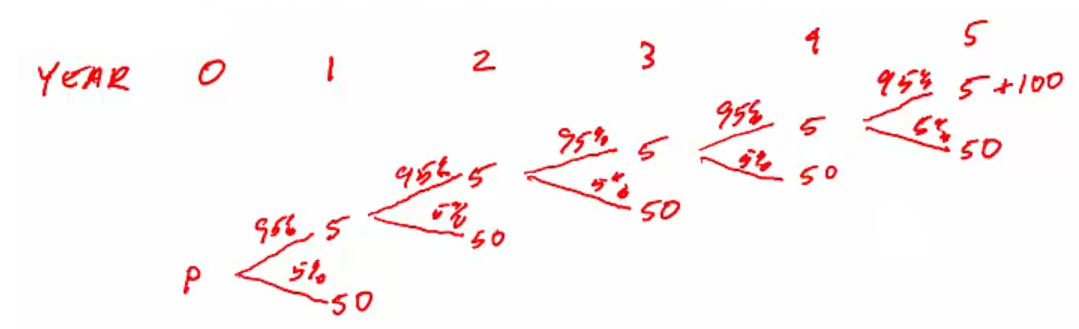
\includegraphics[width=0.6\textwidth]{LECTURE_4/rep5.png}
        \caption{Replicating Portfolio Diagram}
        \label{fig:replicating_portfolio_diagram}
    \end{figure}

    We start from the end and work our way back to find the price of the bond:
    \begin{align*}
        P_{up}^{(4)}   & = 5 + \frac{\mathbb{E}[P^{(5)}]}{1.03} & = 5 + \frac{105\times0.95 + 50.5\times0.05}{1.03} = 104.27 \\
        P_{down}^{(4)} & = 50
    \end{align*}
    Above gives the price at year 4, right when we receive the coupon/payout. We can now find the price at year 3:
    \begin{align}
        P_{up}^{(3)}   & = 5 + \frac{\mathbb{E}[P^{(4)}]}{1.03} & = 5 + \frac{104.27\times0.95 + 50\times0.05}{1.03} = 103.6 \\
        P_{down}^{(3)} & = 50                                                                                                \\
        P_{up}^{(2)}   & = 5 + \frac{\mathbb{E}[P^{(3)}]}{1.03} & = 5 + \frac{103.6\times0.95 + 50\times0.05}{1.03} = 102.41 \\
        P_{down}^{(2)} & = 50                                                                                                \\
    \end{align}
    We can now find the price at year 1, remember, we don't receive a coupon at year 1:
    \begin{align*}
        P_{up}^{(1)} & = \frac{\mathbb{E}[P^{(2)}]}{1.03} & = \frac{102.41\times0.95 + 50\times0.05}{1.03} = 96.88
    \end{align*}

    The yield can be found by:
    \begin{align*}
        P                & = A(P/A, i_{\text{yield}}, N) + F(P/F, i_{\text{yield}}, N) \\
        96.88 = 5(P/A, i_{\text{yield}}, 5) + 100(P/F, i_{\text{yield}}, 5)            \\
        i_{\text{yield}} & = 0.05735
    \end{align*}
\end{example}